\documentclass[tikz,border=10pt]{standalone}
\usepackage{tikz}
\usetikzlibrary{positioning, shapes.geometric, calc, fit} % Add the 'fit' library

\begin{document}
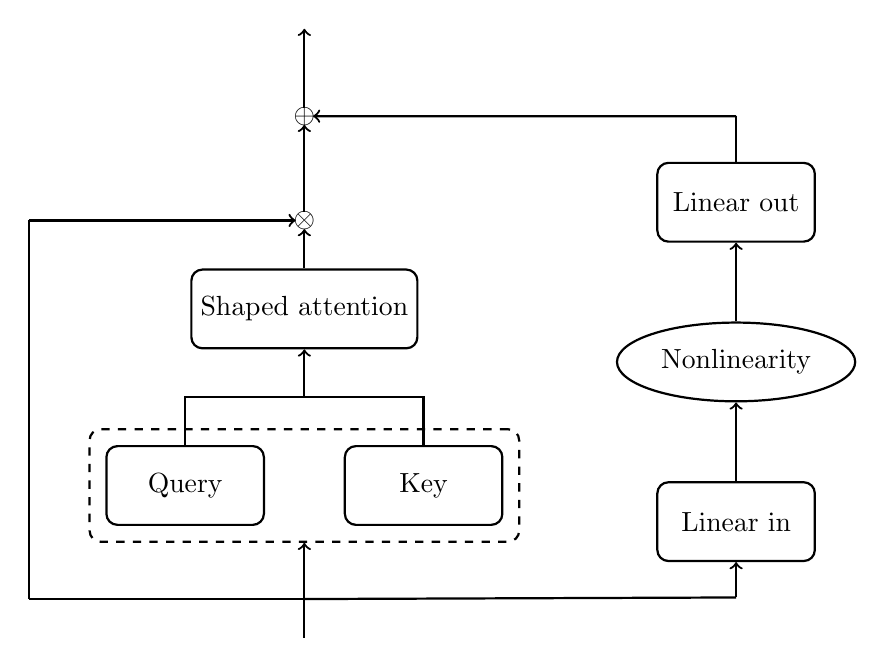
\begin{tikzpicture}[node distance=1cm, every node/.style={draw, thick, rounded corners, minimum width=2cm, minimum height=1cm, align=center}]

    % left attention column
    \node (query) {Query};
    \node (key) [right=of query] {Key};
    \node[dashed, draw, thick, rounded corners, inner sep=0.2cm, fit=(query) (key)] (qk) {};
    \node (attn) [above=of qk] {Shaped attention};
    % draw floating otimes above attention (north + 0.5cm)
    \coordinate (otimes_coord) at ($(attn.north) + (0, 0.5cm)$);
    % otimes symbol without drawing
    \node[inner sep=0pt, outer sep=0pt, draw=none, above=0.11cm of attn] (otimes) {$\otimes$};
    \node[dashed, rounded corners, draw=none, inner sep=0.2cm, fit=(qk) (attn) (otimes)] (attn_block) {};

    % arrow from query and key to attention
    \coordinate (join) at ($($(query.north)!0.5!(key.north)$)!0.5!(attn.south)$);
    \draw[thick, -] (query.north) -- ++(0, 0.62);
    \draw[thick, -] (key.north) -- ++(0, 0.62);
    \draw[thick, ->] (join) -- (attn);
    \draw[thick, -] (query.north |- join) -- (join);
    \draw[thick, -] (key.north |- join) -- (join);
    \draw[thick, ->] (attn) -- (otimes_coord);

    % right mlp column
    \node (act) [right=of attn_block, ellipse, draw, thick, minimum width=2cm, minimum height=1cm, align=center] {Nonlinearity};
    % mlp in (on transformer block level, below act)
    \node (mlp_in) [below=of act] {Linear in};
    \node (mlp_out) [above=of act] {Linear out};
    % invisible box around mlp
    \node[fit=(mlp_in) (act) (mlp_out), inner sep=0pt, draw=none] (mlp_box) {};


    % arrows
    \draw[thick, ->] (mlp_in) -- (act);
    \draw[thick, ->] (act) -- (mlp_out);

    % coordinate for the transformer
    \coordinate (transformer) at ($($(attn_block.east)!0.5!(mlp_box.west)$)!0.5!(attn_block.east)$);

    % weighted addition above attn  
    \coordinate (plus_coord) at ($(attn_block.north) + (0, 0.5cm)$);
    % addition symbol without drawing
    \node[inner sep=0pt, outer sep=0pt, draw=none, above=0.11cm of attn_block] (plus) {$\oplus$};
    % otimes plus 0.11

    \coordinate (otimes_above) at ($(otimes_coord) + (0, 0.22cm)$);
    \draw[thick, ->] (otimes_above) -- (plus_coord);

    % oplus center east
    \coordinate (oplus_center_east) at ($(plus_coord) - (-0.11cm, -0.11cm)$);
    % mlp to oplus (coord above mlp on oplus center east level)
    \coordinate (mlp_above) at ($(mlp_box.north) + (0, 0.565cm)$);
    \draw[thick, ->] (mlp_above) -- (oplus_center_east);
    % line from mlp_out to above mlp
    \draw[thick, -] (mlp_out) -- (mlp_above);


    % coord below attention block
    \coordinate (below_attn) at ($(attn_block.south) - (0, 0.5cm)$);
    % below below attn
    \coordinate (below_below_attn) at ($(below_attn) - (0, 0.5cm)$);
    \draw[thick, -] (below_attn) -- (below_below_attn);
    % below mlp coord (on same level as below_attn)
    \coordinate (below_mlp) at ($(mlp_box.south) - (0, 0.435cm)$);
    % draw line from below mlp to below attn
    \draw[thick, -] (below_mlp) -- (below_attn);

    \draw[thick, ->](below_attn) -- (qk.south);
    \draw[thick, ->](below_mlp) -- (mlp_in.south);

    % coordnidate on bottom line to the left
    \coordinate (left_attn) at ($(below_attn) - (3.5cm, 0)$);
    % draw from below attn to left of attn
    \coordinate (left_above_attn) at ($(otimes_coord) - (3.5cm, -0.11cm)$);
    \draw[thick, -] (below_attn) -- (left_attn);
    \draw[thick, -] (left_attn) -- (left_above_attn);
    \coordinate (oplus_center_west) at ($(oplus_center_east) - (0.22cm, 0)$);
    \draw[thick, ->] (left_above_attn) -- ($(otimes_coord) - (0.11cm, -0.11cm)$);
    % oplus top
    \coordinate (plus_top) at ($(plus_coord) - (0, -0.22cm)$);
    % above above oplus
    \coordinate (above_above_oplus) at ($(plus_top) + (0, 1cm)$);
    \draw[thick, ->] (plus_top) -- (above_above_oplus);
    
    
    


    


    % transformer block
    % \node[draw, thick, rounded corners, inner sep=1cm, fit=(attn_block) (mlp_box) (plus)] (transformer_block) {};


\end{tikzpicture}
\end{document}
